\documentclass[12pt, a4paper]{article}

\usepackage{xeCJK}
\usepackage[margin=2.0cm]{geometry}
\usepackage{fancyhdr}
\usepackage{graphicx}
\usepackage{amsmath, amssymb, amsfonts}
\usepackage{listings} % code showing
\usepackage{pagecolor} % for code color define
\usepackage{tocloft}

% -- 字型
% -- https://www.overleaf.com/help/193#!CJK
% -- https://www.ffonts.net/cwTeXKai.font.download
\setCJKmainfont{cwTeXKai}

% -- 段落格式
\setlength{\headheight}{28pt}
\pagestyle{fancy}
\fancyhf{}
\setlength\parindent{0pt}
\setlength{\parskip}{0.5em}
\setcounter{secnumdepth}{-1}
\renewcommand{\cftsecleader}{\cftdotfill{\cftdotsep}}

% -- 圖, 表標題使用中文取代
\renewcommand{\figurename}{圖}
\renewcommand{\tablename}{表}

% -- 圖、表標題與圖表之間距離
\setlength{\abovecaptionskip}{10pt}
\setlength{\belowcaptionskip}{10pt}

% \renewcommand{\section}[2]{}

% -- 顯示程式碼格式
\definecolor{codegreen}{rgb}{0,0.6,0}
\definecolor{codegray}{rgb}{0.5,0.5,0.5}
\definecolor{codepurple}{rgb}{0.58,0,0.82}
\definecolor{backcolour}{rgb}{0.95,0.95,0.92}
\lstdefinestyle{pystyle}{
    backgroundcolor=\color{backcolour},
    commentstyle=\color{codegreen},
    keywordstyle=\color{magenta},
    numberstyle=\footnotesize\color{codegray},
    stringstyle=\color{codepurple},
    basicstyle=\ttfamily\footnotesize,
    breakatwhitespace=false,
    breaklines=true,
    captionpos=b,
    keepspaces=true,
    numbers=left,
    numbersep=5pt,
    showspaces=false,
    showstringspaces=false,
    showtabs=false,
    tabsize=2,
    extendedchars=false
}
\lstset{style=pystyle}

% ---------------------------------------------

\begin{document}

\chead{\textbf{Ten-Bar Truss Homework}}
\lhead{SOLab}
\rhead{李亭宜}
\cfoot{\thepage}

% \ ~ \

\tableofcontents\thispagestyle{fancy}

\section{Introduction}
In order to minimize the total mass of all elements in ten-bar truss problem, we need to calculate the mass, stress and displacement of each element fist. Then, optimize the problem with matlab.

\section{Ten-Bar Truss Problem}
    \begin{figure}[h]
	\centering
	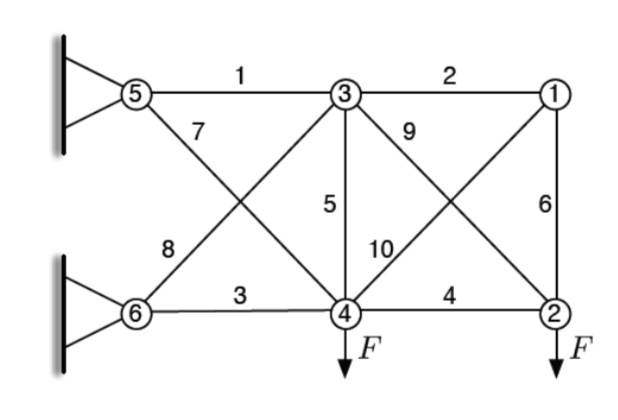
\includegraphics[width=6cm]{./pics/ten-bar truss.png}
	\caption{Ten-Bar Truss  \cite{homework}}
	\label{ten-bar truss}
	\end{figure}
	
\subsection*{Objective}
\begin{itemize}
    \item Calculate total mass of all bars: objective function
    \item Calculate stress in each bar: boundary condition and answer
    \item Calculate displacement of each node: boundary condition and answer
    \item Calculate reaction force: answer
\end{itemize}

\subsection*{Assumption}
\begin{itemize}
    \item Structure in static equilibrium
    \item Each bar treated as two-force member while ignoring the weight
    \item Connection between bars is pin connection
\end{itemize}

\subsection*{Known Conditions}
\begin{itemize}
    \item Structure in static equilibrium
    \item Young's Modulus $E = 200 \ GPA$
    \item Density $\rho = 7860\ kg/m^3$
    \item Yield strength $\sigma_y=250\ MPa$
    \item Length of horizontal and vertical bar $L=9.14\ m$
    \item $r_1 \in $ radius of element 1 to 6\\$r_2 \in$ radius of element 7 to 10
    \item External force at node 2 and 4 with downward direction
\end{itemize}

\section{Ten-Bar Solution}
\qquad Solving ten-bar truss problem will start from filling up the element table. From the information in the element table, we can get the stiffness matrix, which can be used to determine displacement. After knowing the displacement, stress and reaction forces can be calculated.



\subsection{Element Table}
    \qquad First, Filling up element table by defining the nodes and elements.
        \begin{table}[h]
        	\caption{table 1}
        	\label{element table}
        	\centering
        	\begin{tabular}{|c||c|c|c|c|c|c|}
        	\hline
        	{element}& {node 1} & {node 2}&{R}&{L}&{cos}&{sin}\\ \hline
        	\hline
        	1   & 3 & 5 & $r_1$ & 9.14  & -1 & 0 \\ \hline
        	2   & 1 & 3 & $r_1$ & 9.14  & -1 &  0\\  \hline
        	3   & 4 & 6 & $r_1$ & 9.14  & -1 &  0\\  \hline
        	4   & 2 & 4 & $r_1$ & 9.14  & -1 &  0\\  \hline
        	5   & 3 & 4 & $r_1$ & 9.14  & 0  & -1\\  \hline
        	6   & 1 & 2 & $r_1$ & 9.14  & 0  & -1\\  \hline
        	7   & 4 & 5 & $r_2$ & 12.93 & -0.707 & 0.707\\ \hline
        	8   & 3 & 6 & $r_2$ & 12.93 & -0.707 & -0.707\\ \hline
        	9   & 2 & 3 & $r_2$ & 12.93 & -0.707 & 0.707\\ \hline
        	10  & 1 & 4 & $r_2$ & 12.93 & -0.707 & -0.707\\ \hline
        	
        	\end{tabular}
        \end{table}
        
\subsection{Stiffness Matrix}
    \qquad Each of the 6 nodes has 2 DOF, one in x direction and the other in y direction. \\
    \qquad Each element has two nodes, and each node has two DOF. As the result, the stiffness matrix of each element would be in 4 DOF.
        
    \begin{equation}
        k_i = \frac{EA_e}{L_e}
    \left[
        \begin{array}{cccc}
             c^2 &cs &-c^2 & -cs \\
             cs &s^2 & -cs& -s^2 \\
             -c^2& -cs& c^2& cs \\
             -cs & -s^2& cs &s^2
        \end{array}
    \right]
    \end{equation}
        
    \begin{equation*}
        \qquad where
    \left\{
        \begin{array}{c}
            c=cos\theta_i\\
            s=sin\theta_i
        \end{array}
    \right.
        , i=1,2,\ldots,10
    \end{equation*}
        
        
    \qquad By combining stiffness matrices of all ten elements, we can get a 12 DOF stiffness matrix. To check whether the stiffness matrix is correct, we set $r_1=0.1,r_2=0.05$ and check the answer.
    \begin{equation*}
        \mathbf{K}=
        \left[
        \begin{smallmatrix}
            0.7482  &  0.0608  &       0  &       0 &  -0.6874 &        0 &  -0.0608 &  -0.0608 &        0 &        0 &        0 &        0\\
            0.0608 &   0.7482  &       0  & -0.6874 &        0 &        0 &  -0.0608 &  -0.0608 &        0 &        0 &        0 &        0\\
                 0  &       0  &  0.7482  & -0.0608 &  -0.0608 &   0.0608 &  -0.6874 &        0 &        0 &        0 &        0 &        0\\
                 0  & -0.6874  & -0.0608  &  0.7482 &   0.0608 &  -0.0608 &        0 &        0 &        0 &        0 &        0 &        0\\
           -0.6874  &       0  & -0.0608  &  0.0608 &   1.4964 &        0 &        0 &        0 &  -0.6874 &        0 &  -0.0608 &  -0.0608\\
                 0  &       0  &  0.0608  & -0.0608 &        0 &   0.8090 &        0 &  -0.6874 &        0 &        0 &  -0.0608 &  -0.0608\\
           -0.0608  & -0.0608  & -0.6874  &       0 &        0 &        0 &   1.4964 &        0 &  -0.0608 &   0.0608 &  -0.6874 &        0\\
           -0.0608  & -0.0608  &       0  &       0 &        0 &  -0.6874 &        0 &   0.8090 &   0.0608 &  -0.0608 &        0 &        0\\
                 0  &       0  &       0  &       0 &  -0.6874 &        0 &  -0.0608 &   0.0608 &   0.7482 &  -0.0608 &        0 &        0\\
                 0  &       0  &       0  &       0 &        0 &        0 &   0.0608 &  -0.0608 &  -0.0608 &   0.0608 &        0 &        0\\
                 0  &       0  &       0  &       0 &  -0.0608 &  -0.0608 &  -0.6874 &        0 &        0 &        0 &   0.7482 &   0.0608\\
                 0  &       0  &       0  &       0 &  -0.0608 &  -0.0608 &        0 &        0 &        0 &        0 &   0.0608 &   0.0608
        \end{smallmatrix}
        \right]
        \times 10^9
    \end{equation*}
      
\subsection{Determine Displacement} 
    \qquad The relationship between displacement and force can be represented as (\ref{fkq}). \textbf{F} and \textbf{Q} are  $12\times12$ matrices, 
    
    \begin{equation}
        \label{fkq}
        \mathbf{F_{12\times1}=K_{12\times12}\quad Q_{12\times1}}
    \end{equation}
    \begin{equation*}
        \left\{ 
        \begin{array}{ccc}
            f_{2n-1} & \in & \textrm{force in x direction on node n}\\
            f_{2n} & \in & \textrm{force in y direction on node n}\\
            q_{2n-1} & \in & \textrm{displacement in x direction on node n}\\
            q_{2n} & \in & \textrm{displacement in y direction on node n}\\
        \end{array}
        \right.
        \quad n=1,2,\ldots,6
    \end{equation*}
    
    \qquad By applying boundary condition, we know that node 5 and 6 are fixed without displacement. Thus, $q_9=q_{10}=q_{11}=q_{12}=0$. Equation (\ref{fkq}) can now be reduced as (\ref{fkq_re}). The force is applied at node 2 and 4 with downward direction.
    
    \begin{equation}
        \label{fkq_re}
        \mathbf{F_{reduced}=K_{reduced}\quad Q_{reduced}}
    \end{equation}
    
    
    \begin{equation*}
        \mathbf{F}_{reduced}=
        \left[
        \begin{array}{cccc}
            f_1 & f_2 & \cdots & f_8 \\
        \end{array}
        \right]
        ^{T}
    	,
        \left\{
        \begin{array}{l}
        	f_4=f_8=1.0\times 10^7\\
            f_1=f_2=f_3=f_5=f_6=f_7=0
        \end{array}
        \right.
    \end{equation*}
    \begin{equation*}
        \mathbf{K}_{reduced}=
        \left[
        \begin{array}{cccc}
            k_{1,1} & k_{1,2} & \cdots & k_{1,8} \\
            k_{2,1} & k_{2,2} & \cdots & k_{2,8} \\
            \vdots & \vdots & \ddots & \vdots \\
            k_{8,1} & k_{8,2} & \cdots & k_{8,8} \\
        \end{array}
        \right]
    \end{equation*}
    \begin{equation*}
        \mathbf{Q}_{reduced}=
        \left[
        \begin{array}{cccc}
            q_1 & q_2 & \cdots & q_8 \\
        \end{array}
        \right]
        ^{T}
    \end{equation*}
    \\
    \begin{equation}
        \therefore \mathbf{Q_{reduced}=K_{reduced}^{-1}F_{reduced}}
    \end{equation}
        



\subsection{Determine Stress} 
    \qquad With displacement known, we can use (\ref{stress}) to calculate stress in each element.
    \begin{equation}
        \mathbf{\sigma}_{4\times1}=
        \left[
        \begin{array}{c}
             \sigma_{2a-1}  \\\sigma_{2a}\\\sigma_{2b-1}\\\sigma_{2b}
        \end{array}
        \right]
        =\frac{E_i}{L_i}
        \left[
        \begin{smallmatrix}
            -cos\theta_{2a-1}& -sin\theta_{2a}& cos\theta_{2b-1} & sin\theta_{2b}
        \end{smallmatrix}
        \right]
        \left[
        \begin{array}{c}
            q_{2a-1}  \\q_{2a}\\q_{2b-1}\\q_{2b}
        \end{array}
        \right]
        \label{stress}
    \end{equation}
    
    \begin{equation*}
        \left\{
        \begin{array}{l}
            E_i:\textrm{ Young's modulus of element i}\\
            L_i:\textrm{ length of element i}\\
            i=1,2,\ldots,10\\
            a:\textrm{ the first node of element i} \\
            b:\textrm{ the second node of element i} \\
        \end{array}
        \right.
    \end{equation*}


\subsection{Determine Reaction} 
    \qquad Reaction force will appear at fixed node 5 and 6. The corresponding DOFs are DOF9 to DOF12, and the relationship can be expressed as (\ref{reaction}).
    \begin{equation}
        \label{reaction}
        \mathbf{R}_{4\times1}=
        \begin{bmatrix}
           R_{9}\\R_{10}\\R_{11}\\R_{12}
        \end{bmatrix}
        =\mathbf{K}_{reaction}\mathbf{Q}_{12\times1}
    \end{equation}
    \begin{equation*}
        \mathbf{K}_{reaction}=
        \begin{bmatrix}
            k_{9,1} & k_{9,2} & \cdots & k_{9,12} \\
            k_{10,1} & k_{10,2} & \cdots & k_{10,12} \\
            \vdots & \vdots & \ddots & \vdots \\
            k_{12,1} & k_{12,2} & \cdots & k_{12,12} \\
        \end{bmatrix}
    \end{equation*}

\section{Optimize}
    \qquad The optimization can be expressed as (\ref{optimize}).
    \begin{equation}
        \label{optimize}
        \begin{split}
            \min_{r_1,r_2} & \quad f(r_1,r_2)= \sum_{i=1}^{10}m_i(r_1,r_2)\\
            \textrm{subject to} & \quad |\mathbf{\sigma}_i| \leq\sigma_{yield}\\
            & \quad \Delta s_2 \leq 0.02\\
            \textrm{where} & \quad m_i: \textrm{mass of node i}\\
            &\quad \mathbf{\sigma}_i: \textrm{stress in element i}\\
            &\quad \sigma_{yield}: \textrm{yield stress}\\
            &\quad \Delta s_2: \textrm{displacement of node 2}
        \end{split}
    \end{equation}
    \qquad The objective function (\ref{objective}) is the total mass of all elements. For the boundary equation, stress in each element could be determined from (\ref{stress}), while the displacement of node 2 can be calculated from (\ref{fkq_re}).
    \begin{equation}
        \label{objective}
        f(r_1,r_2)= \sum_{i=1}^{10}m_i=\sum_{i=1}^{6}L_{i}\pi r_1^2 \rho + \sum_{i=7}^{10}L_{i}\pi r_2^2 \rho, \quad i=1,2,\ldots,10
    \end{equation}
    \qquad By using the fmincon function in matlab, we get the result as follow:
    \begin{align}
    \label{result}
    \begin{split}
     (r_1,r_2)=&\quad (0.3000,0.2663)\\
    f(r_1,r_2)=&\quad 212410
    \end{split}
    \end{align}
    
\section{Result}
    \qquad From the answer in (\ref{result}), the result of required stress in each bar, displacement of each node, and reaction force at fixed nodes can be calculated.
    \begin{equation}
    	\mathbf{\sigma}=
        \begin{bmatrix}
        	\sigma_1 \\ \sigma_2 \\ \cdots \\ \sigma_{10}
        \end{bmatrix}
        =
        \begin{bmatrix}
        	6.9286\\    1.4647\\   -7.2163  \\ -2.0715  \\  1.3209  \\  1.4647  \\  6.6079 \\  -6.0913\\ 3.7195   \\-2.6301
        \end{bmatrix}
        \times 10^7 (Pa),\textrm{\quad where}
        \left\{
        \begin{array}{l}
        \sigma_i: \textrm{stress in element i}\\
        i=1,2,\ldots,10
        \end{array}
        \right.
    \end{equation}
    \begin{equation}
    	\mathbf{Q}=
        \begin{bmatrix}
        	q_1 \\ q_2 \\ \cdots \\q_{12}
        \end{bmatrix}
        =
        \begin{bmatrix}
        	0.0038\\
           -0.0189\\
           -0.0042\\
           -0.0195\\
            0.0032\\
           -0.0087\\
           -0.0033\\
           -0.0093\\
                 0\\
                 0\\
                 0\\
                 0
        \end{bmatrix}
        (m)
        ,\textrm{\quad where}
        \left\{
        \begin{array}{l}
        q_{2n-1}: \textrm{displacement in x direction of node n}\\
        q_{2n}: \textrm{displacement in y direction of node n}\\
        n=1,2,\ldots,6
        \end{array}
        \right.
    \end{equation}
    \begin{equation}
    	\mathbf{R}=
        \begin{bmatrix}
           R_{9}\\R_{10}\\R_{11}\\R_{12}
        \end{bmatrix}
        =
        \begin{bmatrix}
        	-3.0000\\
            1.0407\\
            3.0000\\
            0.9593
        \end{bmatrix}
        \times10^7
        (N)
        \textrm{,\quad where}
        \left\{
        \begin{array}{l}
        R_{2n-1}: \textrm{reaction force in x direction of node n}\\
        R_{2n}: \textrm{reaction force in y direction of node n}\\
        n=5,6
        \end{array}
        \right.
    \end{equation}



\section{References}
% -- 隱藏預設參考文獻標題
\begingroup
    \renewcommand{\section}[2]{}
    \bibliographystyle{ieeetr}
    \bibliography{ref.bib}
\endgroup

\end{document}